% =============================================================================
% Title:        Transfer tank
% Author:       Nathaniel Thomas
% Affiliation:  Texas A&M University, Department of Nuclear Engineering
% Email:        nathaniel@tamu.edu
% Date Created: 3/18/2026
% Version:      1.0
%
% Description:
%   A .tex source file describing the transfer tank for the salt purifier.
%
% =============================================================================

\section{Transfer tank}

Following purification, the salt is transferred to the transfer tank using
positive pressure. The transfer tank is a CF-flanged stainless steel
316L tank. It has a lid on top with three \SI{0.5}{in} tubes. One tube is
for purging, another is for pulling vacuum, and the central tube is for
salt transfer. The transfer tank is shown in \Cref{fig: transfer tank}. \par

\begin{figure}
  \centering
  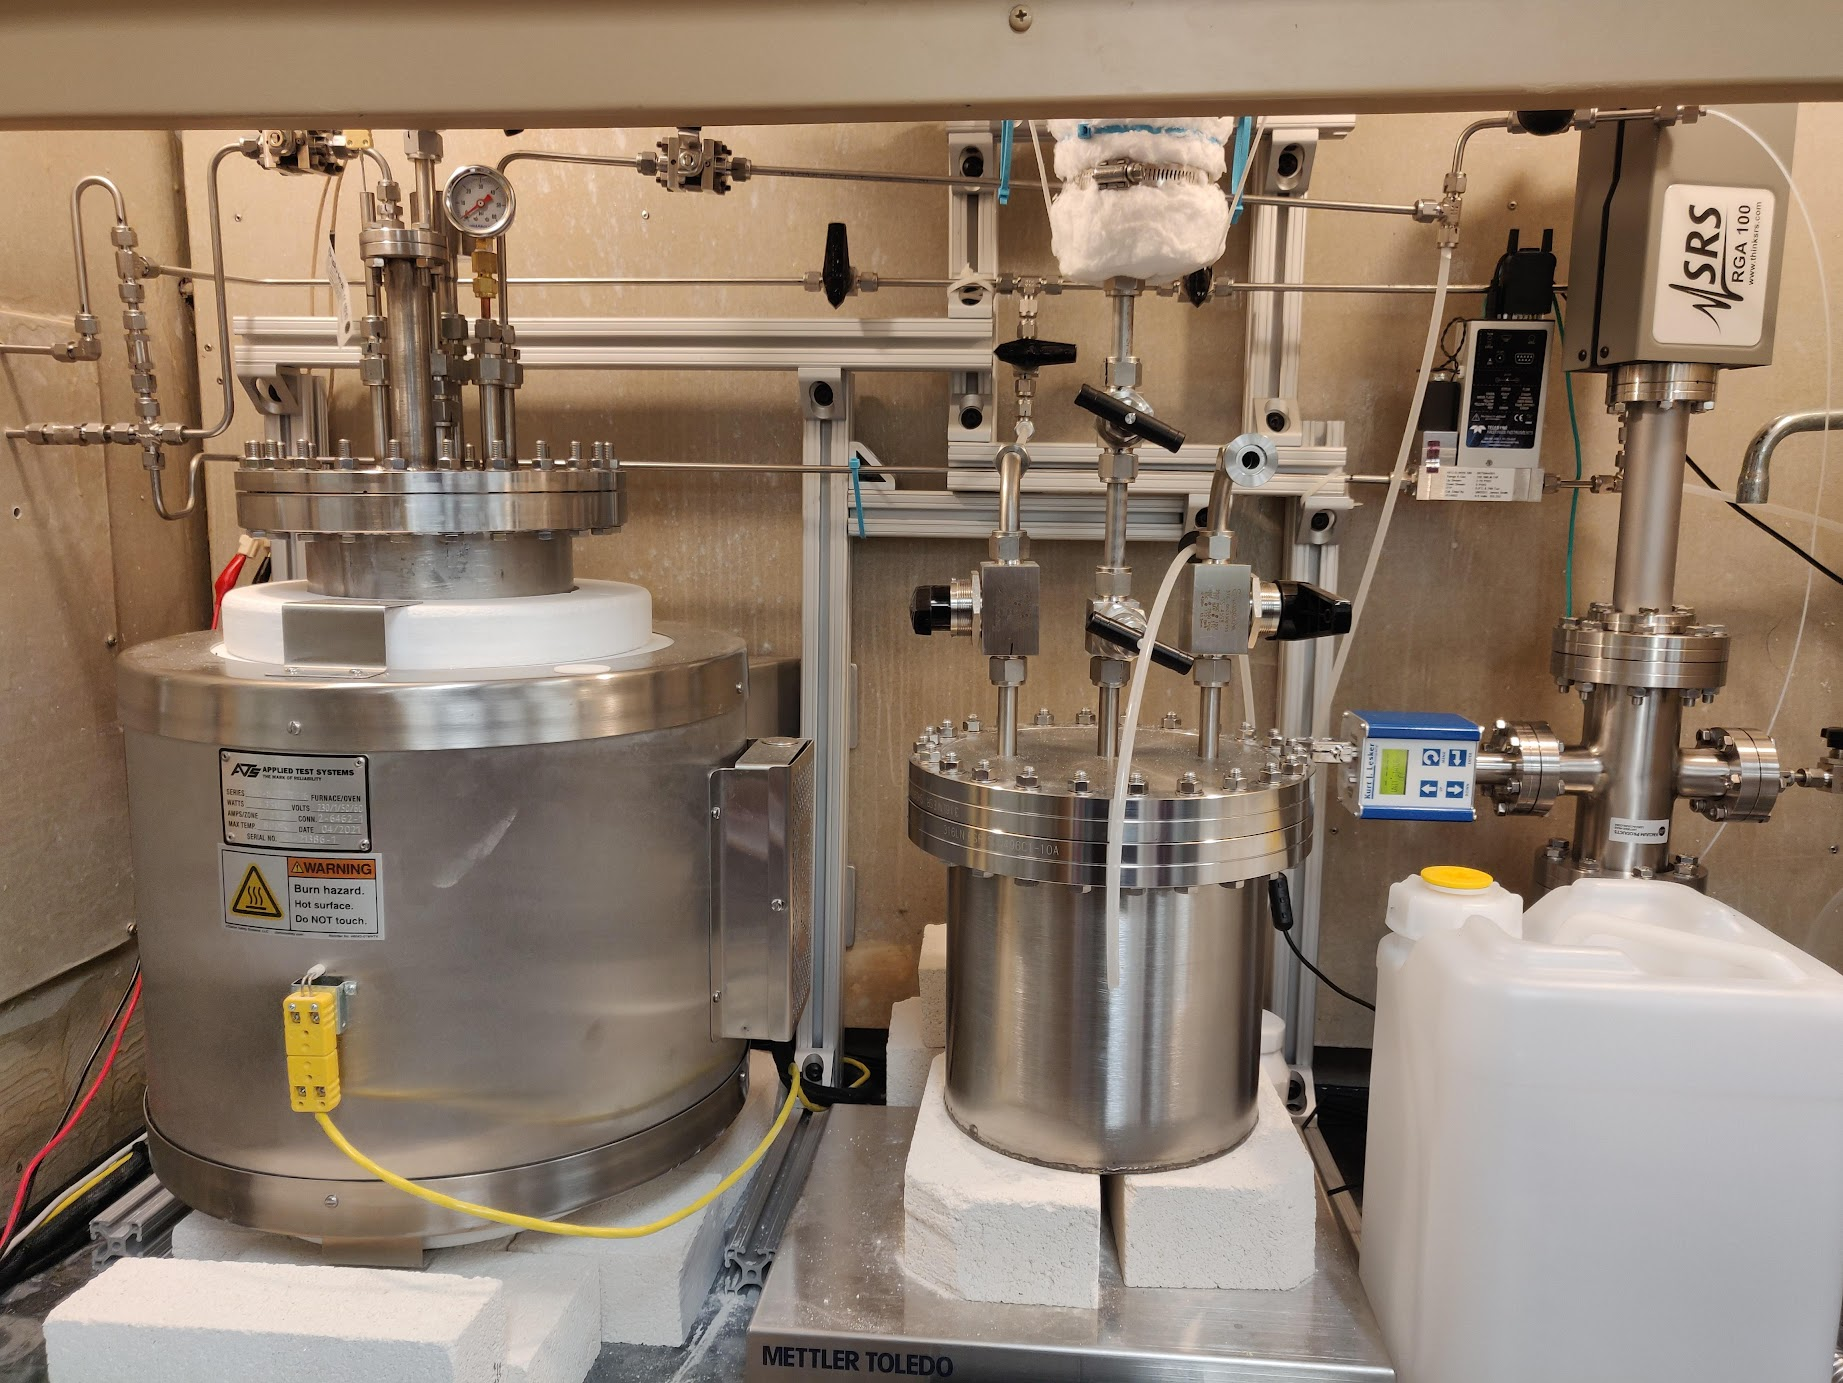
\includegraphics[width=0.6\textwidth]{./assets/pictures/transfer tank.png}
  \caption{Am image of the transfer tank (11/22/2022).}
  \label{fig: transfer tank}
\end{figure}

\subsection{Transfer tank base}

The transfer tank base is a 316L stainless steel tank with a CF flange.
It is shown in \Cref{fig: transfer tank base}.

\begin{figure}
  \centering
  \includegraphics[width=0.6\textwidth]{./assets/pictures/cleaned
  transfer tank bottom.jpg}
  \caption{Am image of the transfer tank base (1/23/2026).}
  \label{fig: transfer tank}
\end{figure}

\subsection{Transfer tank lid}

The transfer tank lid is a 316L stainless steel tank with a CF flange.
It is shown in \Cref{fig: transfer tank base}.

\begin{figure}
  \centering
  \includegraphics[width=0.6\textwidth]{./assets/pictures/finished
  and welded transfer tank lid top.jpg}
  \caption{Am image of the transfer tank lid (2/28/2026).}
  \label{fig: transfer tank}
\end{figure}
